% Définitions de la class
\documentclass[12pt]{article}

% Import du template
\usepackage{template_cr}
\usepackage[ruled,vlined]{algorithm2e}

% Définition des variables d'environnement
\makeatletter
	\title{TP 3 - Programmation Réseau}	\let\Title\@title
	\author{Etienne RICHARD, Matthieu CIZDZIEL et Mathis MOGUEDET} \let\Author\@author
	\date{\today}           	\let\Date\@date
	\newcommand{\UE}{Attaque par cannaux auxiliaires : Cryptanalyse du système RSA}
\makeatother

% Retirons les indentations des paragraphes
\setlength{\parindent}{0pt}

% Commande de compilation : 
% pdflatex -shell-escape rapport.tex ; pdflatex -shell-escape rapport.tex
\begin{document}
\maketitle
\pagebreak

\tableofcontents
\pagebreak

\section*{Introduction}
\addcontentsline{toc}{section}{Introduction}

\section{Contexte du projet}
\subsection{Introduction}
En terme de sécurité informatique les méthodes de chiffrement sont très importantes notamment dans le domaine des télécommunication. La cryptographie est donc une notion très importante dans la cybersécurité actuelle. Les 3 principes de la cryptographie sont la confidentialité, l'authenticité et l'intégrité.
La confidentialité assure que le contenu d'un message chiffré ne peut être lu que par son destinataire.
L'authenticité assure l'origine du message, c'est à dire l'identité du messager.
Enfin l'intégrité assure la non-modification d'un message.
Dans notre cas nous mettrons en oeuvre des moyens pour s'attaquer à la confidentialité d'un protocole cryptographique. 
Ainsi nous allons vous présenter un algorithme connu pour sa robustesse et utilisé dans le monde entier, le protocole RSA.
% \newpage
\subsection{Généralités sur le RSA}
Nous ne pouvons pas commencer la présentation du projet sans présenter le protocole RSA.
Le protocole RSA utilise une clé publique pour chiffrer le message et une clé privé pour le déchiffrer. Les clés publique et privé n'étant pas les mêmes, on parle de chiffrement asymétrique.
La robustesse du RSA repose dans la difficulté de factoriser un produit de deux grands nombres premiers.
Sans rentrer dans le détail de sa robustesse nous allons vous expliquer son fonctionnement:
\\

\textbf{Génération des clés}


Soit $p$ et $q$ deux nombres premiers distincts. On pose alors $n=pq$ et $\phi(n)=(p-1)(q-1)$.
On choisit ensuite un nombre $e$ premier avec $\phi(n)$ et strictement inférieur à $\phi(n)$
On peut enfin calculer $d$ l'inverse modulaire de $e$ modulo $\phi(n)$.
Ainsi le couple (n,e) constitue la clé publique et $d$ la clé privée. Nous pouvons rapidement nous rendre compte qu'il n'est pas possible d'obtenir $d$ sans connaitre la factorisation de $n$, c'est pourquoi on dit que le RSA repose sur un problème de factorisation.
\\

\textbf{Chiffrement}


Soit un message représenté par un entier naturel m strictement inférieur à n et c le message chiffré.
Nous avons la relation suivante:
\begin{equation}
\label{eq:chiffrement}
c \equiv m^e [n]
\end{equation}
Ainsi pour chiffrer un message m on utilise une fonction d'exponentiation modulaire utilisant la clé publique.
\\

\textbf{Déchiffrement}


Nous pouvons de la même manière déchiffrer le message chiffré à l'aide de la clé privée. 
Nous avons ainsi la relation suivante :
\begin{equation}
\label{eq:dechiffrement}
m \equiv c^d [n]
\end{equation}


Ainsi nous remarquons que la base du chiffrement et du déchiffrement repose sur une exponentiation modulaire. Le problème de l'exponentiation utilisé par le RSA est qu'elle ne peut pas être naïve, c'est à dire qu'on ne peut pas faire $ x^n = x*x*x...*x$ n fois. En effet, le RSA utilise des nombres de 2048 bits ce qui rend impossible l'utilisation d'un algorithme naïf.
Nous verrons par la suite lors de l'implémentation du RSA qu'on peut utiliser l'algorithme d'exponentiation rapide pour des nombres de 2048 bits.
% \newpage
\subsection{Attaques par canaux auxiliaires}
Il est désormais temps de vous introduire au concept d'attaque par canaux auxiliaires.
Selon Wikipedia \cite{wki:sca} une attaque par canaux auxiliaires est une:
"Attaque informatique qui, sans remettre en cause la robustesse théorique des méthodes et procédures de sécurité, recherche et exploite des failles dans leur implémentation, logicielle ou matérielle."
En reprenant ce que nous vous avons présenter précédemment nous ne remettons pas en compte la robustesse du protocole RSA mais son implémentation utilisant l'algorithme d’exponentiation rapide.
Ainsi il existe une multitude d'attaques par canaux auxiliaires comme les attaques temporelles basées sur le temps mis par l'algorithme pour effectuer certaines opération, les attaques pas sondage qui consiste à analyser un circuit en y posant une sonde ou encore les attaques par consommation de courant.
Dans notre cas nous allons nous intéresser aux attaques par consommation de courant. Ces attaques sont basées sur le fait que chaque type d'opération que peut effectuer le processeur utilise plus ou moins de courant. On peut également généraliser ce principes pour les différentes fonctions d'un programme qui n'ont pas la même consommation électrique.
% \newpage
\subsection{Matériel utilisé}
Nous pouvons désormais présenter le matériel utilisé dans ce projet. Nous utiliserons un kit ChipWhisperer de la marque NewAE prêtée par notre tuteur M. Guy Goniat. Ce kit est composé de trois cartes différentes :
\begin{itemize}
\item Une carte cible qui fera tourner le firmware cible, c'est à dire le firmware implémentant le RSA;
\item Une carte mère CW308 sur laquelle nous branchons la carte cible, cette carte permet d'alimenter la carte cible;
\item Une carte d’acquisition servant d'interface entre l'ordinateur et la carte mère.Cette carte permet d'uploader le firmware sur la carte mère, de communiquer avec la carte cible et de récupérer la consommation de courant de la carte cible sur l'ordinateur
\end{itemize}
\pagebreak
Nous pouvons nous aider de la figure ci-dessous pour mieux comprendre l’organisation des différents composants:
\begin{figure}[H]
    \centering
    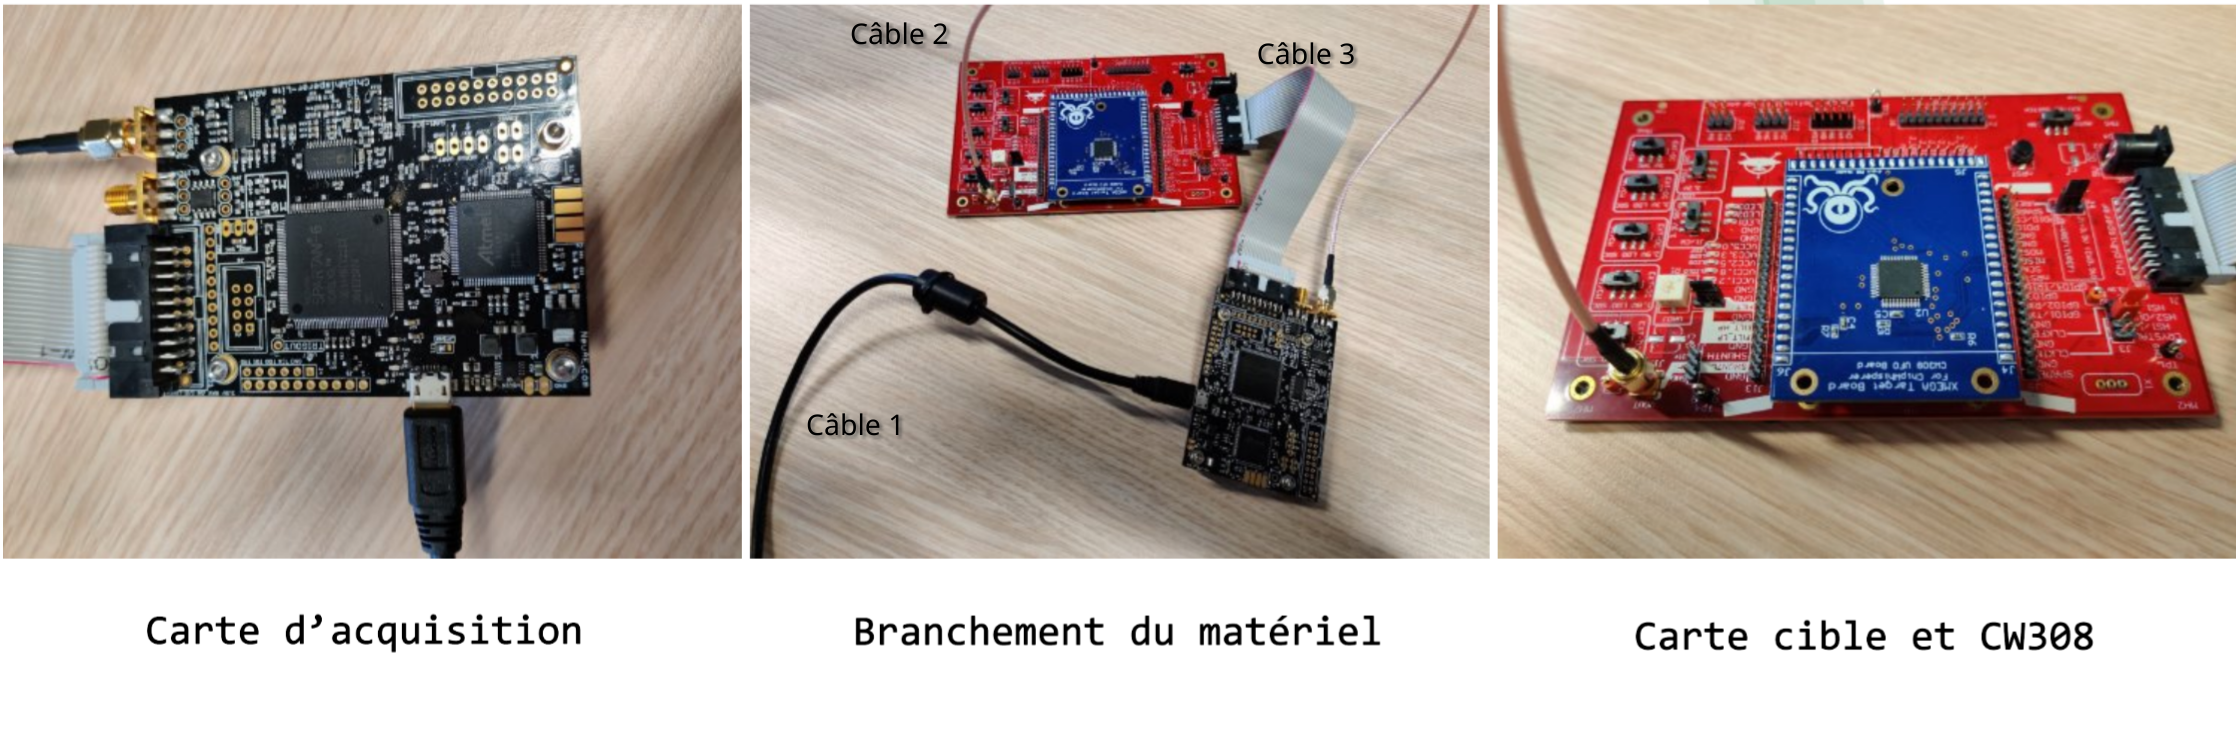
\includegraphics[width=\textwidth]{fig/materiel.png}
    \caption{Matériel utilisé pour le projet}
    \label{fig:materiel}
\end{figure}

Nous pouvons voir sur cette image 3 câbles différents. Le câble 1 permet de communiquer entre l’ordinateur et la carte d’acquisition. Il permet également d'alimenter l'ensemble du kit ChipWhisperer. Le câble 2 permet de récupérer la consommation du courant de la carte cible. Enfin le câble 3 permet de transmettre les informations entre la carte mère et la carte d’acquisition.
Nous utiliserons également la librairie ChipWhisperer pour mener à bien ce projet.
% \newpage
\subsection{Enjeux et objectifs du projet}
Nous connaissons désormais tous les éléments nécessaires à la compréhension des enjeux et des objectifs de notre projet. L'objectif principal de ce projet est de récupérer la clé privée d'un utilisateur sans la connaitre, tout en restant dans un cadre légal. De ce fait nous attaquerons notre propre plateforme dédiée aux attaques par canaux auxiliaires. Les enjeux liés à ce projet sont nombreux, il faudra réussir à s’organiser autour d'un projet en équipe, comprendre le fonctionnement du kit ChipWhisperer et de la librairie associée et respecter les deadlines du planning établit lors de l'étude projet.

\subsection{Conclusion}
Ce projet vise ainsi à attaquer un protocole de cryptographie, le RSA, connu et utilisé pour sa robustesse. Cela sera possible grâce à l'implémentation du RSA et grâce à l'utilisation de matériels dédié à ce genre d'attaque. Un travail en équipe et une forte rigueur seront important dans ce projet puisque ce dernier est conséquent. Nous pouvons désormais nous intéresser un peu plus en détail à l'implémentation du RSA dans ce projet. 



\section{Implémentation du RSA}
\input{sections/2_implémentation_du_rsa}

\section{Attaque}
\subsection{Introduction}
Dans cette partie nous allons voir comment l'attaque par analyse de consommation a été mise en place, c'est à dire comment fonctionne notre kit ChipWhisperer et ce que nous avons fait dessus. Ceci comprend l'explication des firmwares, l'obtention et l'analyses des résultats obtenus.

\subsection{Installation de la ChipWhisperer (CW)}
Tout d'abord, nous avons pris en main le matériel, nous avons donc découvert les différentes cartes qui étaient à notre disposition dans le kit fournit.
Deuxièmement, nous avons branché physiquement la carte d'acquisition à un ordinateur via un port USB, c'est cette carte qui nous enverra la consommation de notre cible.

Nous nous sommes ensuite penché sur la connexion avec un ordinateur, afin de pouvoir communiquer avec la ChipWhisperer. Nous avons du chercher longuement afin de trouver comment nous connecter à cette carte via l'ordinateur. Pour ce faire, nous avons principalement consulté le wiki ChipWhisperer et d'autres forums afin de trouver une solution. 
Nous avons donc commencé par installer les différents packages nécessaires pour utiliser la carte. Cette partie fut compliqué car le guide d'installation de la ChipWhisperer n'expliquait pas la marche à suivre pour nos OS respectifs. Cependant il était écrit qu'il était tout de même possible d'installer les paquets nécessaires au fonctionnement de la carte. Il a ainsi fallut installer chaque paquets un par un en trouvant le bon paquet disponible sur nos distributions. 

Ensuite nous avons installé JupyterNotebook, qui est un outil simple et accessible pour visualiser et organiser notre connexion et notre communication avec la carte. 
Il nous permettais de lancer chaque commande séparément et d'avoir le retour de la carte en conséquence.
Nous devions aussi utiliser un environnement python spécifique à l'aide de "pyenv" pour que notre JupyterNotebook fonctionne correctement.

\subsection{Fonctionnement de la ChipWhisperer (CW)}
Lorsque la carte a été connectée avec sucés, nous avons eu besoin de connaitre les différentes commandes associés à cette carte afin de faire ce que nous voulions dessus.
Nous nous donc reportés au wiki de cette section qui est : http://wiki.newae.com/SimpleSerial .
La carte communique donc en SimpleSerial, le protocole de communication utilisé pour presque tous les démonstrations de ChipWhisperer.
\icon{Capture_commandes_SimpleSerial.png}

\subsection{Introduction avec un firmware déjà fait}
Maintenant que nous pouvons communiquer avec notre carte, et que nous possèdons les commandes associés à ce firmware, nous avons pu tester les attaques pré-enregistrées dans la carte. 
Nous avons donc testé une attaque classique sur le RSA, grace aux commandes suivantes: 
On va chercher le bon firmware qui correspond à une attaque sur le RSA et on identifie le type de carte cible qui est connecté physiquement.
hardware\victims\firmware\simpleserial-rsa
make PLATFORM=CW303
Ensuite, nous utilisons une fonction qui permet de définir une commande dans ce firmware. 
simpleserial_addcmd('t', 0,  real_dec);
Envoyer la lettre 't' depuis l'odinateur va donc appeler la fonction real_dec (Vrai déchiffrement).



Avec ces commandes, nous avons donc eu des traces de consomations qui nous permetais de retrouver la clé privée qui a été utilisée lors de ce chiffrement RSA.
\subsection{Conception de notre firmware}
Précédemment, nous utilisions un firmware déjà créer par ChipWhisperer, c'est à dire que toutes les fonction de bases pour implémenter le RSA étaient déjà faites, nous n'avions pu qu'à les utiliser. L'avantage d'utiliser son propre firmware est de se mettre en conditions réelles, de pouvoir effectuer toutes les opérations voulues et de les implémenter sous même.
Dans cette partie, nous allons voir comment nous avons créer nos propres fonction avec nos propres commandes.

\subsection{Cryptanalyse}
Une fois que nous avions les traces de consomations, nous devons les exploitées afin de retrouver la clé privée utiliser et donc retrouver le message en clair. 
Dans nos traces, comme notre fonction qui lit les valeurs de consomation commence de la fin, nous devons lire à partir de la fin dans notre trace, ce qui correspond au début de nos valeurs. 
Ensuite, nous devons réussir à identifer des patterns visuellement, c'est a dire des formes qui se répettent dans notre graphique. 
Apres cela, nous devions tester les formes si elles correspondaient à un 0 ou un. Nous essayons de déchiffer le message avec les deux clés obtenues et nous regardions quelle clé était la bonne.
\subsection{Automatisation}
La partie automatisation est assez importante car si nous devions déchiffer sur 2048 bits, c'est à dire analyser une trace qui comprendrais 2048 pics de consomations différents, visuellement, la tache s'averrerait longue et fastidieuse. L'automatisation d'une recherche de clés est donc essentielle et nous permet de gagner du temps d'analyse.
Pour cette automatisation, nous avons choisis de la réaliser en python car ce language possède de nombreuses biliothèques et nous semblait adéquat pour cette partie.
Afin de réaliser l'automatisation, nous avons commencer par ranger les valeurs de consomations dans un tableau. 
Ensuite nous avons commencer par améliorer la lisibilité de notre trace grace un algorithme de lissage de courbe ...
Enfin, lorsque la courbe est lisée nous pouvions utiliser l'algorithme de Person qui permet, une fois le partern trouvé, donner un coefficient de corrélation entre ce qu'il est en train de parcourir est le partern définis.

\subsection{Validation de l'automatisation}
Afin de valider notre automatisation, 
\subsection{Conclusion}
En conclusion la partie attaque de ce projet a été la partie finale 


\section*{Conclusion}
\addcontentsline{toc}{section}{Conclusion}

\end{document}
